\documentclass[11pt]{beamer}

\usetheme{CambridgeUS}
\usecolortheme{dolphin}

\usepackage[utf8]{inputenc}
\usepackage[L7x]{fontenc}
\usepackage[lithuanian]{babel}

\usepackage{amsmath}
\usepackage{amsfonts}
\usepackage{amssymb}
\usepackage{graphicx}


\usepackage{booktabs}
\usepackage{longtable}
\usepackage{array}
\usepackage{multirow}
\usepackage{wrapfig}
\usepackage{float}
\usepackage{colortbl}
\usepackage{pdflscape}
\usepackage{tabu}
\usepackage{threeparttable}
\usepackage{threeparttablex}
\usepackage[normalem]{ulem}
\usepackage{makecell}
\usepackage{xcolor}

\usepackage{hyperref}
\hypersetup{
  colorlinks=true,
  linkcolor=black,
  filecolor=blue,   
  urlcolor=blue,
  citecolor=blue
}

\author{Armintė G. Justas M. Tomas D.}
\title{Title}
\subtitle{subtitle}
%\setbeamercovered{transparent} 
%\setbeamertemplate{navigation symbols}{} 
%\logo{} 
%\institute{Corona-Stat.lt} 
%\date{} 
%\subject{AAA} 

\graphicspath{{./figures/}}


\begin{document}

\begin{frame}
\titlepage
\end{frame}

\begin{frame}
\tableofcontents
\end{frame}

\section{Intro}
\begin{frame}{Corona-Stat.lt projektas}
\begin{itemize}
\item Pirminis tikslas COVID19 plitimo prognozė
\item Komanda (Armintė, Rokas, Tomas)
\item SAM'o nulinė reakcija
\item Nuo COVID19 statistikos link ekonominių įžvalgų
\end{itemize}
\end{frame}


\begin{frame}{Apie COVID prognozavimą}
\begin{itemize}
\item Kaip prognozuojamos epi- ir pandemijos
\item Modelių patikimumas
\item \href{https://mif.vu.lt/lt3/dokumentai/dokumentai/Naujienos/COVID/2020-04-15_SEIR_ilgalakes_prognozes.pdf}{Lietuviški mokslininkai "prognozuoja"}
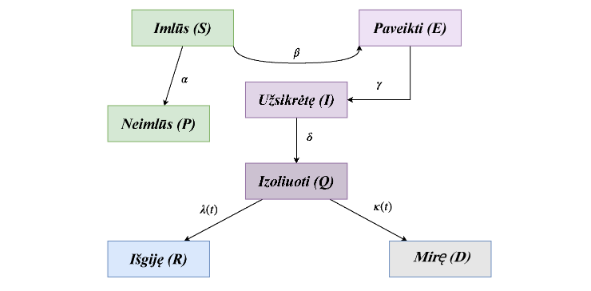
\includegraphics[scale=0.5]{seiqrdp.png}
\item Duomenų atvirumas  
\end{itemize}
\end{frame}

\section{Covid situacija}
\begin{frame}{Covid situacija}

\end{frame}


\section{Nedarbas Lietuvoje}

\begin{frame}{Bedarbių skaičius}
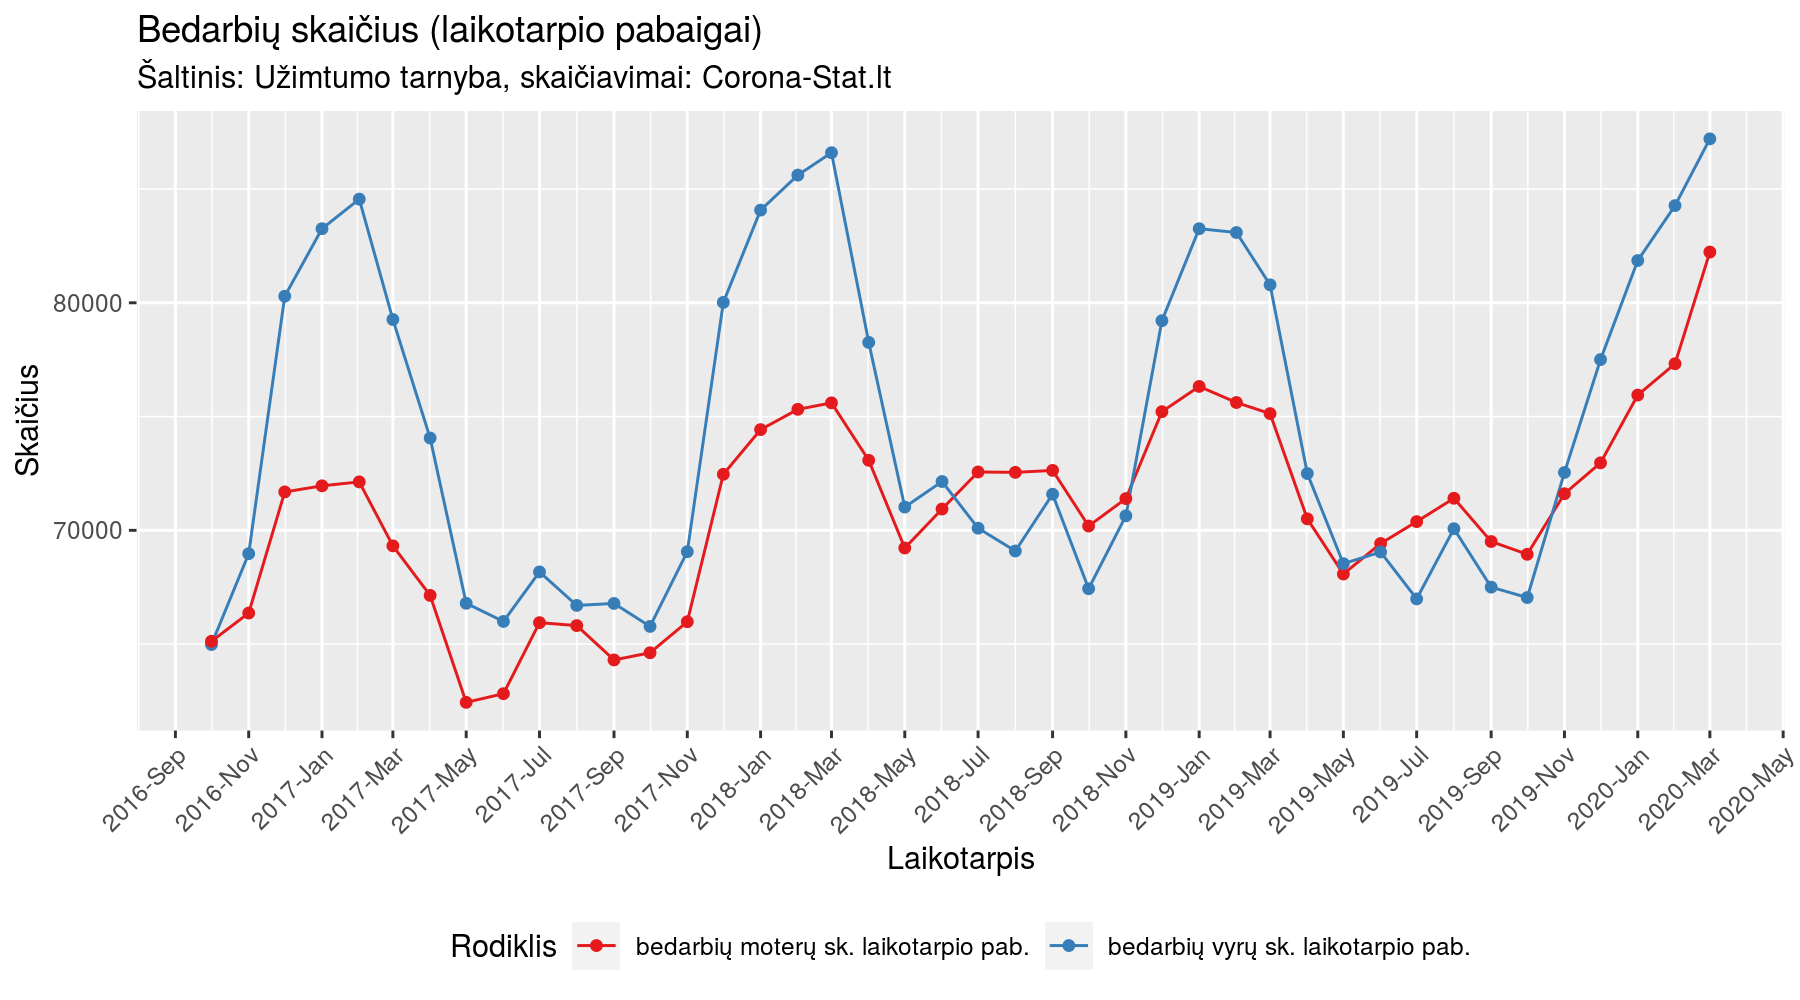
\includegraphics[scale=0.5]{bedarbiu_sk.png}
\end{frame}

\begin{frame}{Bedarbių proc. nuo DAG}
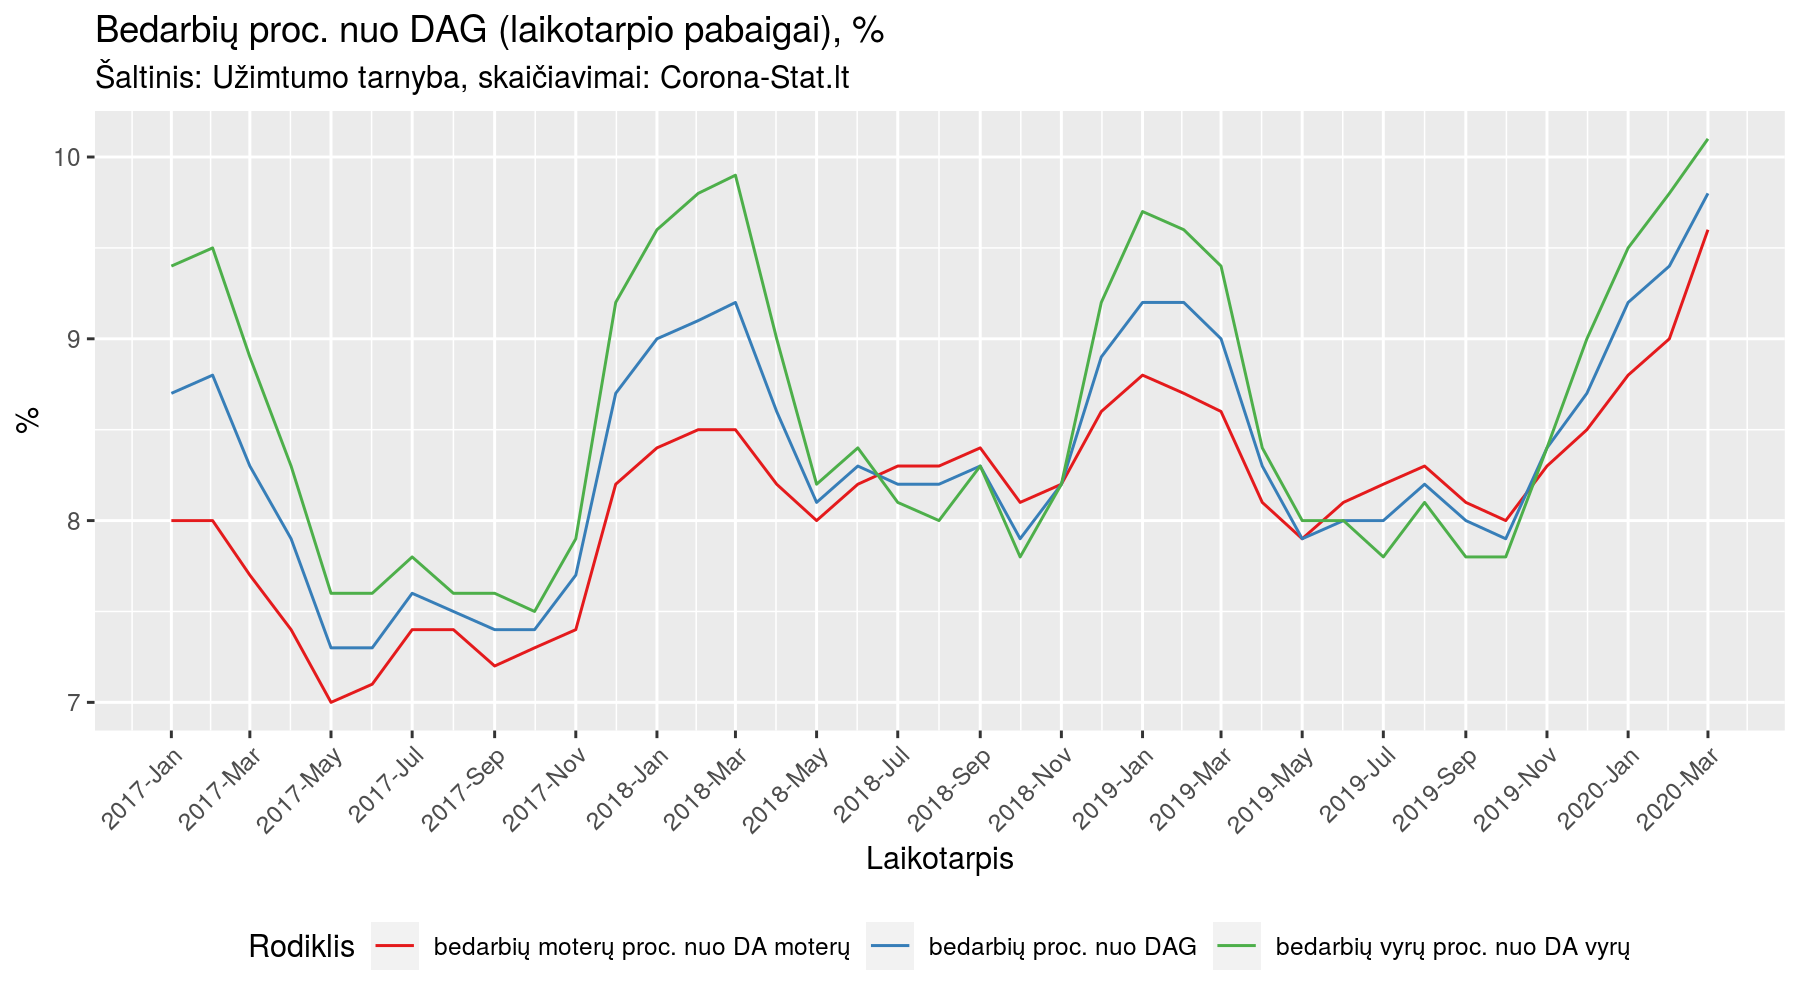
\includegraphics[scale=0.5]{bedarbiu_proc.png}
\end{frame}


\begin{frame}{Grupės darbuotojų atleidimai}
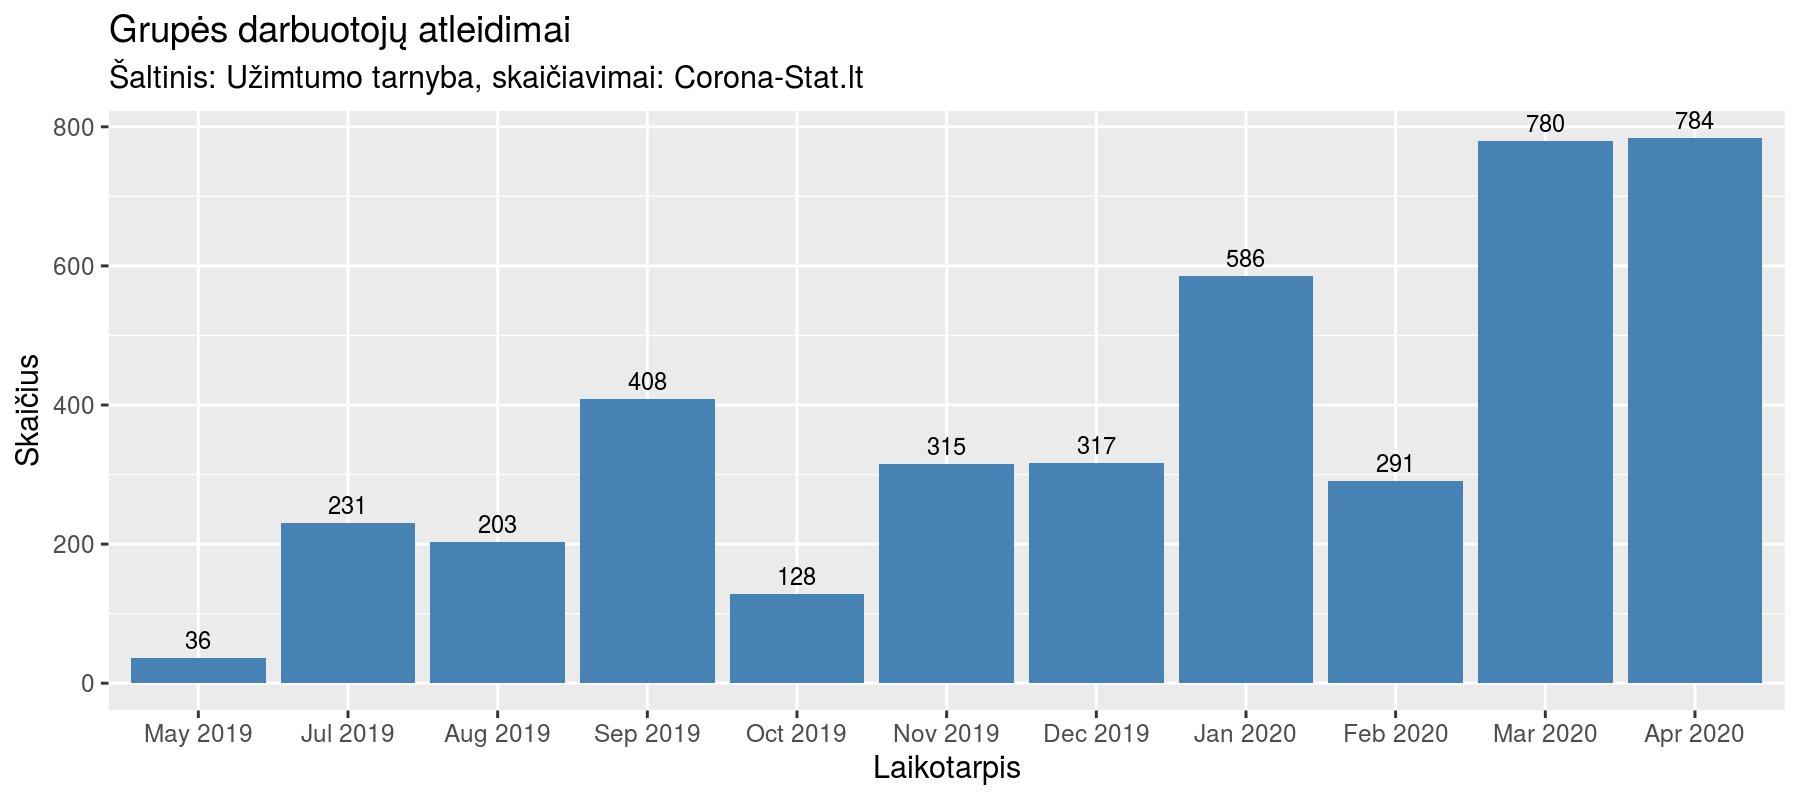
\includegraphics[scale=0.5]{grupes_darbuotoju_atleidimai_men_sum.png}
\end{frame}


\begin{frame}{Grupės darbuotojų atleidimai}

Grupės darbuotojų atleidimai nuo 2020 vasario mėn.
\input{grupiniai_atleidimai.txt}
\end{frame}


\section{Infliacija}
\begin{frame}{Eurozonos metinė infliacija}
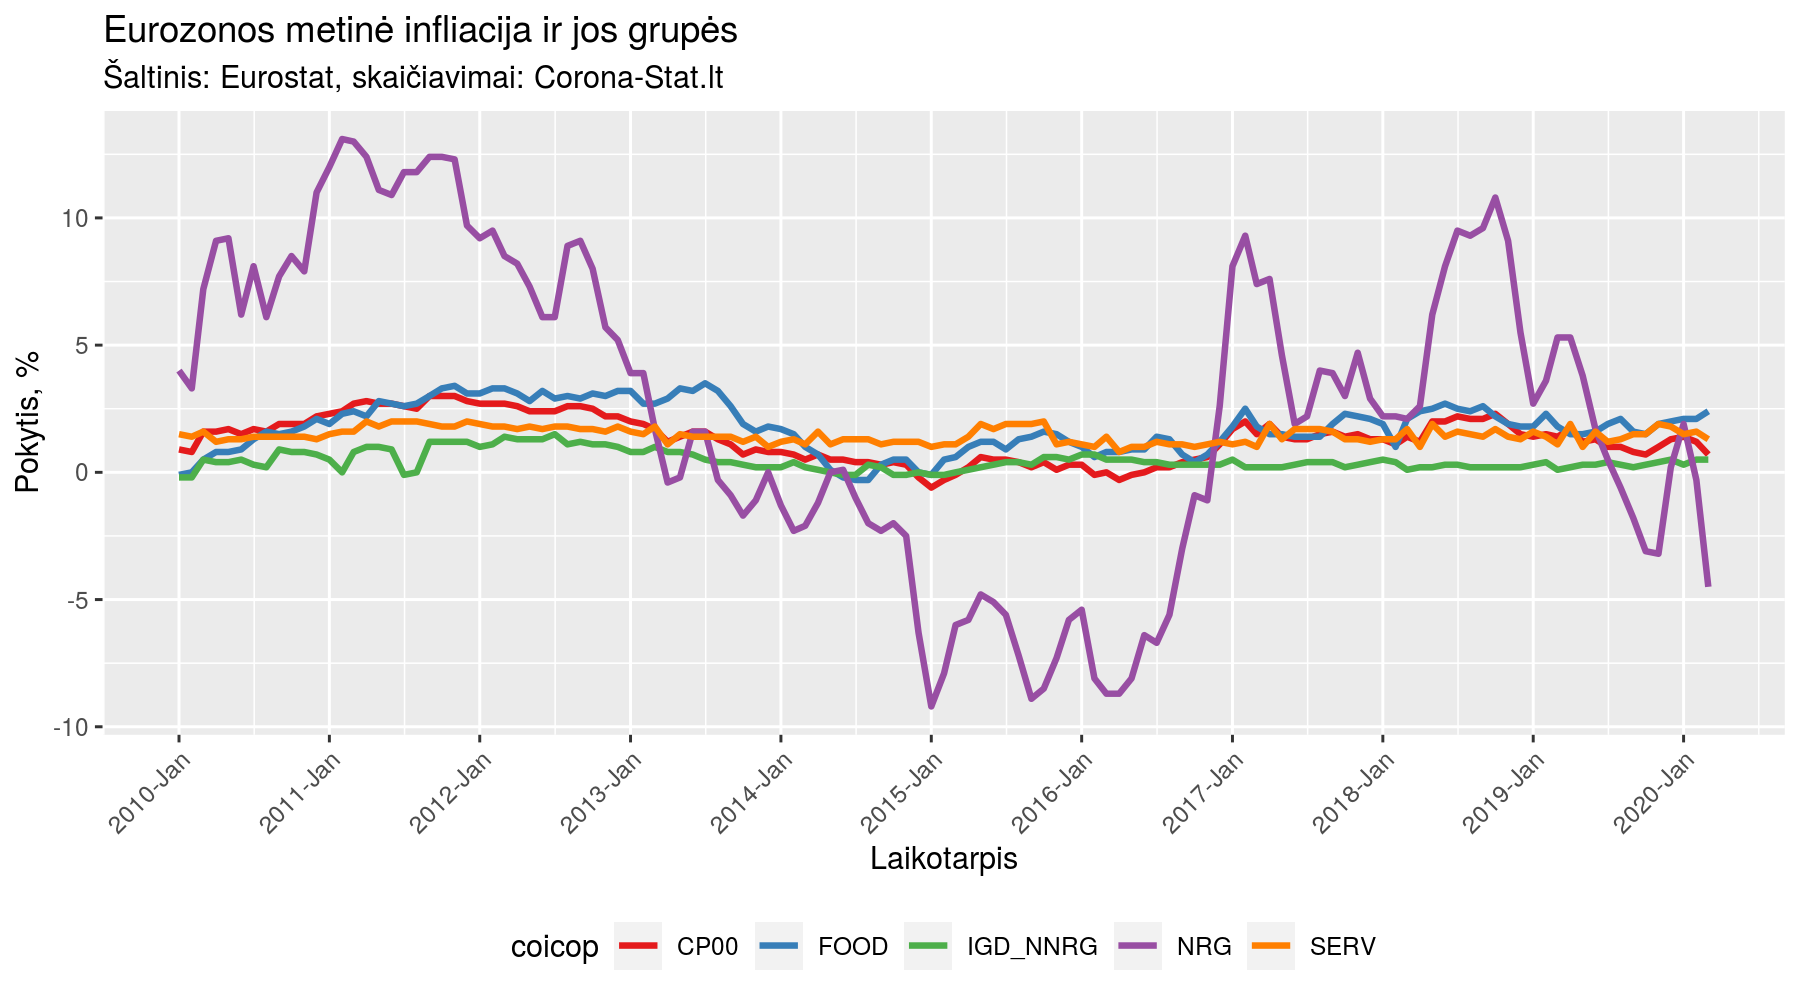
\includegraphics[scale=0.5]{infliacija_ez.png}
\end{frame}

\begin{frame}{Eurozonos metinė infliacija}
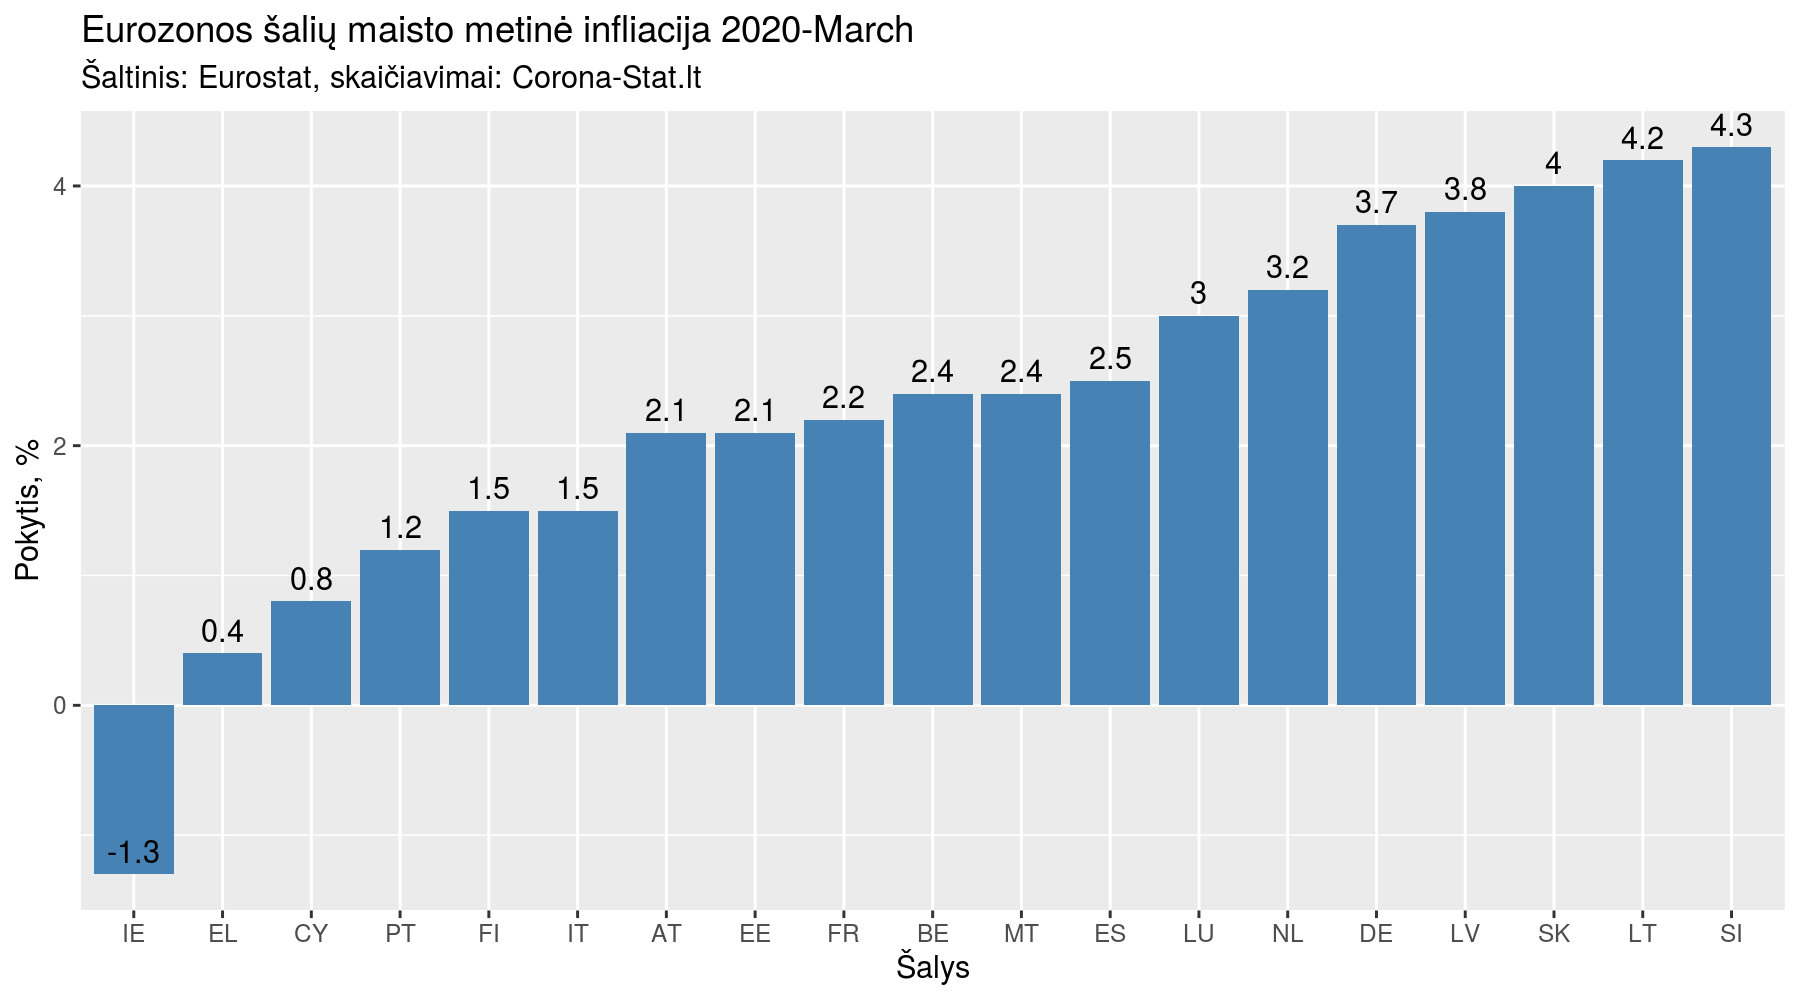
\includegraphics[scale=0.5]{infliacija_maistas.png}
\end{frame}

\begin{frame}{Eurozonos metinė infliacija}
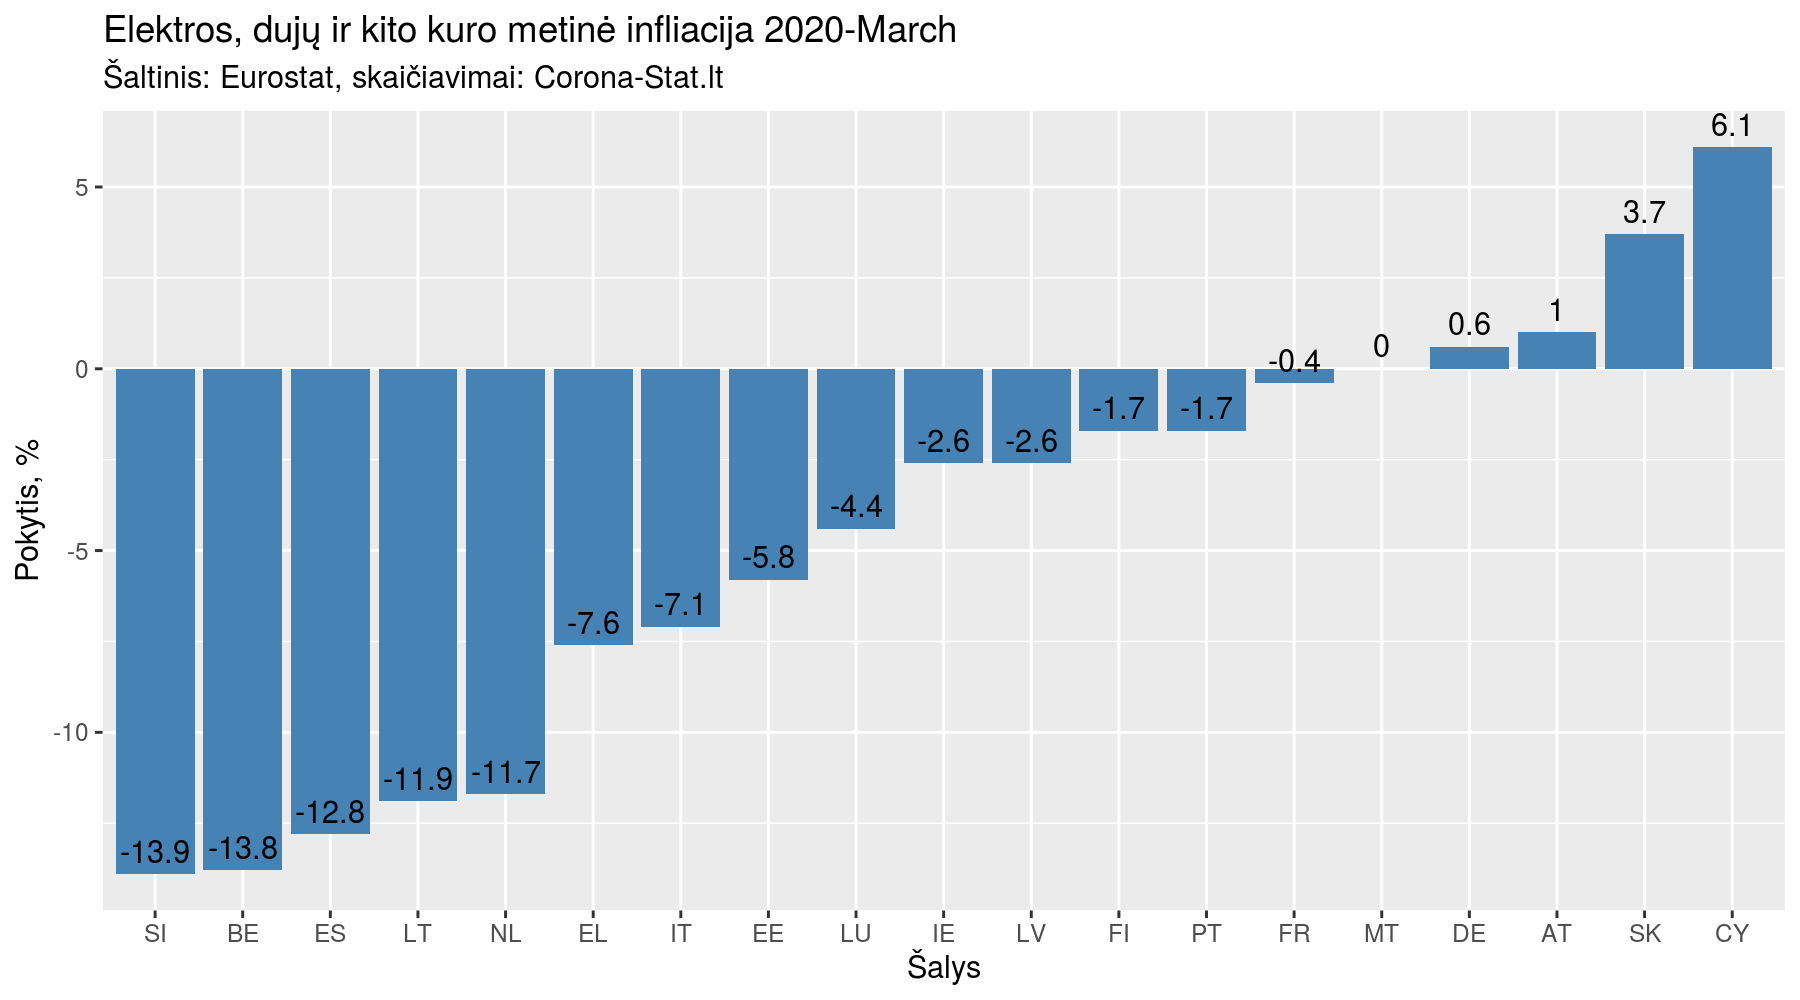
\includegraphics[scale=0.5]{infliacija_elektra_dujos.png}
\end{frame}


\begin{frame}{Eurozonos metinė infliacija}
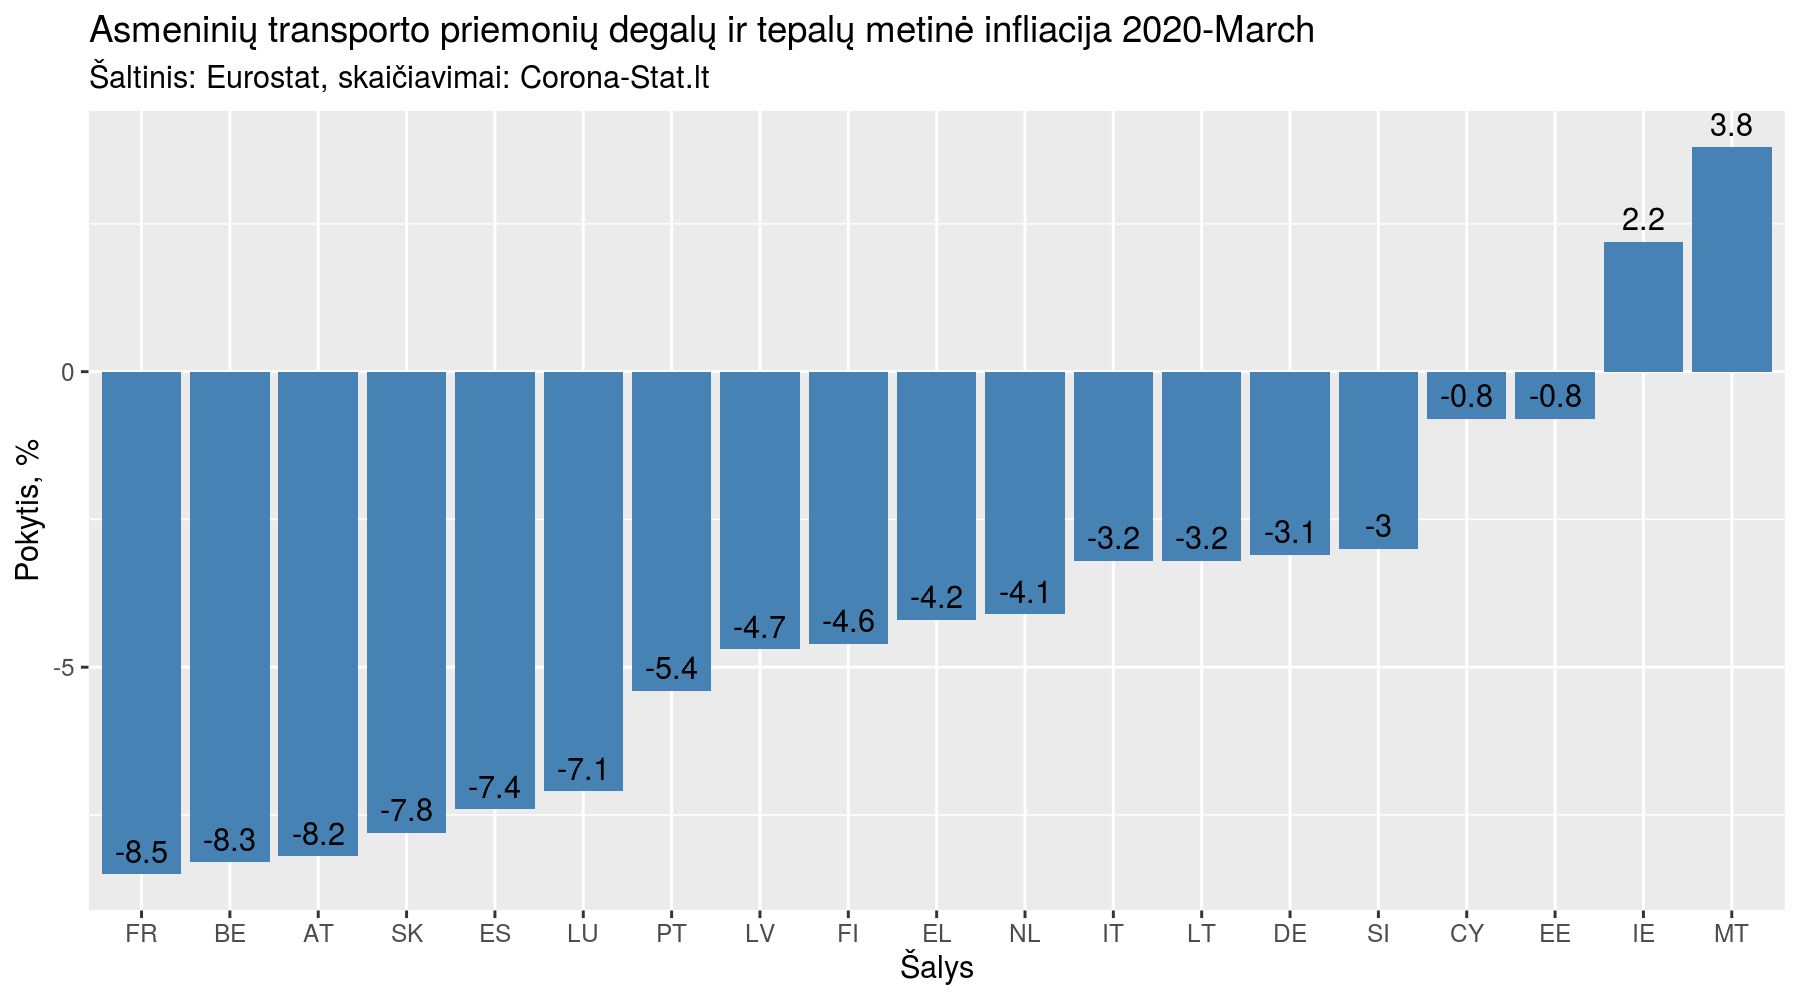
\includegraphics[scale=0.5]{infliacija_degalai.png}
\end{frame}


\section{Apie elektrą ir naftą}
\begin{frame}{Ką rodo elektros suvartojimas Lietuvoje?}
\end{frame}

\begin{frame}{Naftos kaina ir jos poveikis geopolitikai}
\end{frame}

\begin{frame}{Lietuvos elektros ir šildymo kainos 2020H2}
\end{frame}

\section{Pramonė, lūkesčiai, eksporto rinkos}
\begin{frame}{Lietuvos pramonės pokytis 2020M3}
\end{frame}

\begin{frame}{Lietuvos pramonė + verslo lūkesčiai}
\end{frame}

\begin{frame}{Lietuvos eksporto rinkų PMI}
\end{frame}

\begin{frame}{Ar COVID19 sugriaus Europą?}
Kodėl coronabonds o ne ESM
\end{frame}


\section{Koronabonds}

\begin{frame}{Ar COVID19 sugriaus Europą?}
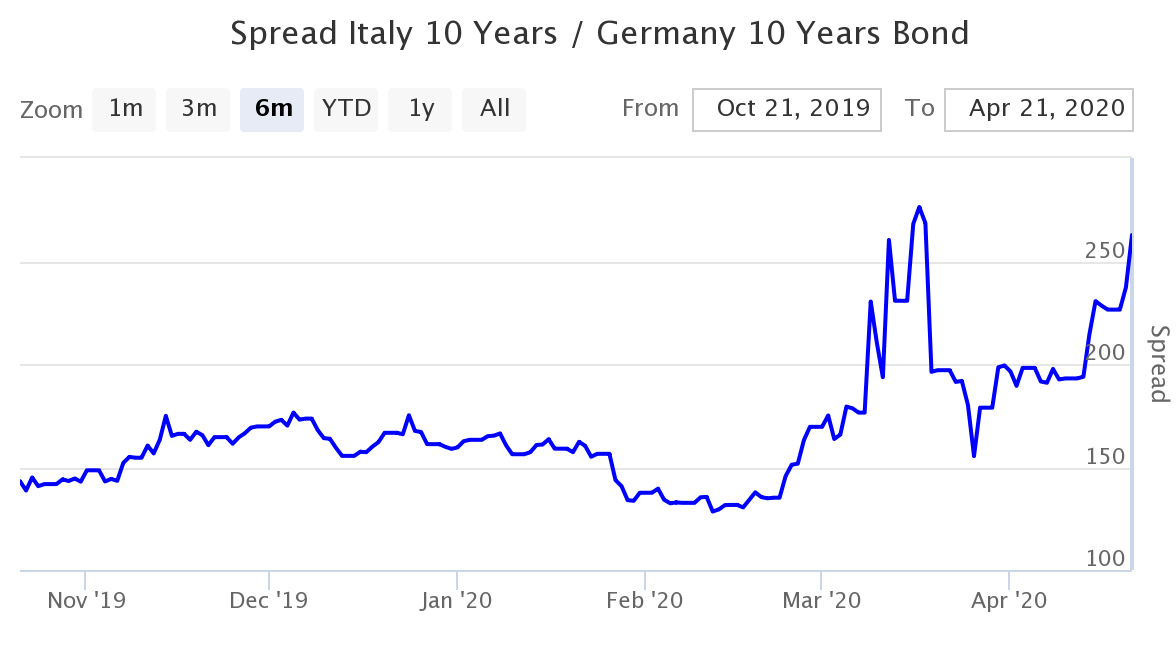
\includegraphics[scale=0.25]{spread-italy-10-years-ge.png}
http://www.worldgovernmentbonds.com/spread/italy-10-years-vs-germany-10-years/
\end{frame}

\end{document}